\documentclass[ 12pt ]{article}
\usepackage{amsmath, amsthm, amssymb, csquotes, bbold, enumitem, extpfeil, graphicx, listings, mathrsfs, tikz-cd}
\usepackage[margin=0.5in]{geometry}
\graphicspath{ ./ }

\begin{document}

\noindent Landon Fox \\
\noindent Math 731, Modern Algebra \\
\noindent September 8, 2021

\begin{center}
\Large Homework 1
\end{center}

\begin{enumerate}
	% problem 1
	\item[\textbf{1.}] Let $X$ be a non-empty set and let $2^X$ be its power set. On $2^X$, define the binary operation $+$ and $\cdot$ as $$A + B = (A - B) \cup (B - A)\;\; \mathrm{and}\;\; A \cdot B = A \cap B.$$ Show that $(2^X, +, \cdot)$ is a commutative ring with identity. Find all zero divisors.

		\begin{proof}
			Provided the construction $(2^X, +, \cdot)$ defined above, we will first show that $(2^X, +)$ is an abelian group. It is easy to see that $+$ is a closed operation. To illustrate associativity, we utilize Venn diagrams; observe that for sets $A, B, C \in 2^X$,
			\begin{center}
				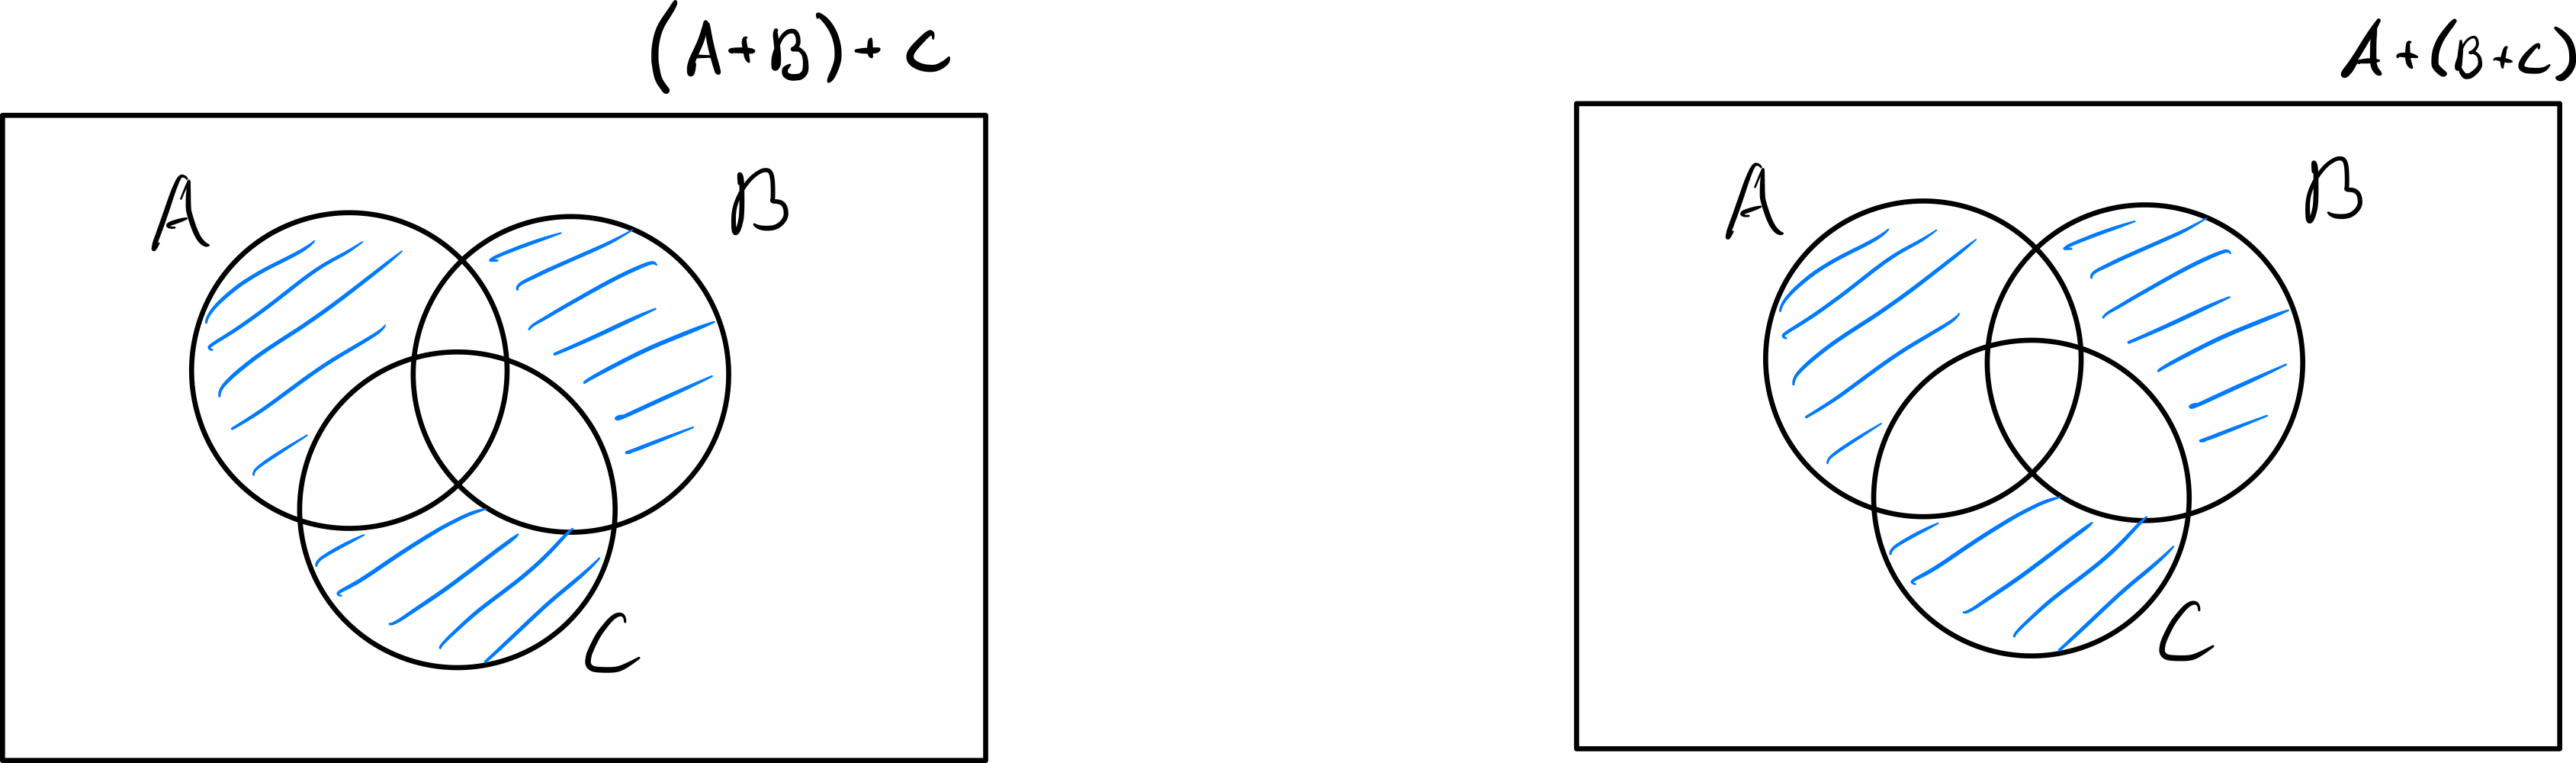
\includegraphics[width=17cm, height=5cm]{File_000}
			\end{center}
			therefore, $(A + B) + C = A + (B + C)$. It is clear that $+$ is an abelian operation due to the commutativity of the union of sets and so it suffices to construct a one sided identity and inverses. Moreover, for any subset $A \subseteq X$, it holds that $$A + \varnothing = (A - \varnothing) \cup (\varnothing - A) = A \cup \varnothing = A,$$ thus $\varnothing$ is the identity of $(2^X, +)$. As for inverses, take a subset $A \subseteq X$, then $$A + A = (A - A) \cup (A - A) = \varnothing \cup \varnothing = \varnothing$$ illustrating that $(-A) = A$. Hence, $(2^X, +)$ is an abelian group by definition. \\

			In regard to multiplication, it is clear that it is also closed and abelian due to the commutativity of the intersection between sets. Hence, we will show only left distributivity: let $A, B, C \in 2^X$, then it follows that
			\begin{align*}
				A \cdot (B + C) &= A \cap ((B - C) \cup (C - B)) \\
				&= (A \cap (B - C)) \cup (A \cap (C - B)) \\
				&= (A \cap B - A \cap C) \cup (A \cap C - A \cap B) \\
				&= (A \cdot B - A \cdot C) \cup (A \cdot C - A \cdot B) \\
				A \cdot (B + C) &= A \cdot B + A \cdot C
			\end{align*}
			provided the distributivity of set intersection and union as well as distributivity of the set intersection and set subtraction. Next, notice that $$A \cdot X = A \cap X = A$$ for any subset $A \subseteq X$ demonstrating that the multiplicative identity of $2^X$ is $X$. Thus, $(2^X, +, \cdot)$ is a commutative ring with identity. \\

			Lastly, we determine all zero divisors of $2^X$. By definition, for a set $\varnothing \neq A \subseteq X$ to be a zero divisor, there must exist a set $\varnothing \neq B \neq X$ such that $A \cap B = \varnothing$. Therefore, $B \subseteq X - A$ and such a $B$ exists if and only if $\varnothing \neq A \subset X$.
		\end{proof}


	% problem 2
	\item[\textbf{2.}] Show that every Boolean ring $R$ is commutative and that $a + a = 0$ for all $a \in R$.

		\begin{proof}
			Let $R$ be a Boolean ring; that is, $a^2 = a$ for all $a \in R$. Consider an element $a \in R$, observe that
			\begin{align*}
				a + a &= (a + a)^2 \\
				&= a^2 + a^2 + a^2 + a^2 \\
				a + a &= a + a + a + a \\
				0 &= a + a;
			\end{align*}
			moreover, $a$ is its own additive inverse. To show commutativity, let $a, b \in R$, then $$a + b = (a + b)^2 = a^2 + ab + ba + b^2 = a + ab + ba + b$$ which provides $ab + ba = 0$. Furthermore, due to uniqueness of additive inverses, it must follow that $ab = ba$.
		\end{proof}


	% problem 3
	\item[\textbf{3.}] Find an example of a ring $R$ with identity and an element $a \in R$ that is left-invertible but not right-invertible.

		\begin{proof}
			Let $(M, e, \cdot)$ be a monoid with presentation consistent with the identity as well as a single relation $ba = e$ for particular $e \neq a, b \in M$. Now, consider the group ring $\mathbb{Z}[M]$. Observe that the element $1 \cdot a \in \mathbb{Z}[M]$ has left-inverse $1 \cdot b$ since $$(1 \cdot b) \cdot (1 \cdot a) = (1 \cdot 1) \cdot (b \cdot a) = 1 \cdot e.$$ However, no right-inverse exists illustrated by the fact that $$(1 \cdot a) \cdot (n \cdot c) = (1 \cdot n) \cdot (a \cdot c) = n \cdot (a \cdot c) \neq 1 \cdot e$$ for all $n \in \mathbb{Z}$ and $c \in M$ via the presentation of $M$.
		\end{proof}


\end{enumerate}

\end{document}
